\documentclass[11pt,letterpaper]{article}

%% ---------- Encoding ----------
\usepackage[T1]{fontenc}
\usepackage[utf8]{inputenc}
\usepackage[english]{babel}

%% ---------- Page geometry ----------
\usepackage[letterpaper,top=0.85in,bottom=1in,left=0.85in,right=0.85in,headheight=14pt]{geometry}

%% ---------- Fonts ----------
\usepackage{lmodern}
\usepackage{helvet}
\renewcommand{\familydefault}{\sfdefault}
\usepackage[scaled=0.92]{inconsolata}

%% ---------- Colors ----------
\usepackage[table]{xcolor}
\definecolor{brandNavy}{HTML}{0B3A6B}
\definecolor{brandBlue}{HTML}{1F6FB2}
\definecolor{brandSky}{HTML}{5AA8E0}
\definecolor{brandLight}{HTML}{F4F7FB}
\definecolor{brandBorder}{HTML}{D8D8D8}
\definecolor{brandRowAlt}{HTML}{F4F7FB}
\definecolor{brandText}{HTML}{1A1A1A}
\definecolor{brandMuted}{HTML}{555555}
\definecolor{brandCodeBg}{HTML}{F5F7FA}
\definecolor{brandCodeRule}{HTML}{D8E1EB}

%% ---------- Packages ----------
\usepackage{graphicx}
\usepackage{tikz}
\usetikzlibrary{arrows.meta,positioning,shapes.geometric,calc,backgrounds,fit}
\usepackage{tabularx}
\usepackage{array}
\usepackage{longtable}
\usepackage{enumitem}
\usepackage{titlesec}
\usepackage{fancyhdr}
\usepackage{tocloft}
\usepackage{caption}
\usepackage{tcolorbox}
\tcbuselibrary{breakable,skins,listings}
\usepackage{lastpage}
\usepackage{float}
\usepackage[hidelinks]{hyperref}

%% ---------- Hyperref ----------
\hypersetup{
  colorlinks=true,
  linkcolor=brandBlue,
  urlcolor=brandBlue,
  citecolor=brandBlue
}

%% ---------- Section styling ----------
\titleformat{\section}
  {\color{brandNavy}\sffamily\Large\bfseries}
  {\thesection.}{0.6em}{}
  [\vspace{2pt}{\color{brandBlue}\titlerule[2.5pt]}]

\titleformat{\subsection}
  {\color{brandBlue}\sffamily\large\bfseries}
  {\thesubsection}{0.55em}{}

\titleformat{\subsubsection}
  {\color{brandNavy}\sffamily\normalsize\bfseries}
  {\thesubsubsection}{0.55em}{}

\titlespacing*{\section}{0pt}{16pt}{8pt}
\titlespacing*{\subsection}{0pt}{12pt}{4pt}
\titlespacing*{\subsubsection}{0pt}{8pt}{2pt}

%% ---------- Page header / footer ----------
\pagestyle{fancy}
\fancyhf{}
\renewcommand{\headrulewidth}{0pt}
\fancyfoot[C]{\small\color{brandMuted}\thepage\ /\ \pageref{LastPage}}
\fancyhead[R]{\small\color{brandMuted}\docrunningtitle}

\fancypagestyle{plaincover}{%
  \fancyhf{}\renewcommand{\headrulewidth}{0pt}}

%% ---------- Lists ----------
\setlist[itemize]{leftmargin=1.4em,itemsep=2pt,topsep=4pt}

%% ---------- Tables ----------
\newcolumntype{L}[1]{>{\raggedright\arraybackslash}p{#1}}
\newcolumntype{C}[1]{>{\centering\arraybackslash}p{#1}}
\newcolumntype{Y}{>{\raggedright\arraybackslash}X}
\renewcommand{\arraystretch}{1.25}
\setlength{\arrayrulewidth}{0.4pt}
\arrayrulecolor{brandBorder}

\newcommand{\thead}[1]{\textcolor{white}{\bfseries #1}}

%% ---------- Code block ----------
\usepackage{listings}
\lstdefinestyle{plain}{
  basicstyle=\ttfamily\small,
  breaklines=true,
  breakatwhitespace=false,
  columns=fullflexible,
  keepspaces=true,
  showstringspaces=false,
  upquote=true,
  literate={->}{{$\rightarrow$}}1 {<-}{{$\leftarrow$}}1,
}
\lstset{style=plain}
\newtcblisting{codeblock}{
  enhanced, breakable,
  colback=brandCodeBg,
  colframe=brandCodeRule,
  boxrule=0.4pt,
  arc=2pt,
  left=8pt, right=8pt, top=6pt, bottom=6pt,
  borderline west={2pt}{0pt}{brandBlue},
  before skip=8pt, after skip=8pt,
  listing only,
  listing options={style=plain},
}

%% ---------- Caption styling ----------
\captionsetup{
  font={small,it,color=brandMuted},
  labelfont={bf,color=brandNavy},
  labelsep=endash,
  skip=4pt
}

%% ---------- TOC styling ----------
\renewcommand{\cftsecfont}{\sffamily\bfseries\color{brandNavy}}
\renewcommand{\cftsecpagefont}{\sffamily\bfseries\color{brandNavy}}
\renewcommand{\cftsubsecfont}{\sffamily\color{brandText}}
\renewcommand{\cftsubsecpagefont}{\sffamily\color{brandMuted}}
\setlength{\cftbeforesecskip}{6pt}
\setlength{\cftbeforesubsecskip}{2pt}
\renewcommand{\contentsname}{\color{brandNavy}\sffamily Table of Contents}

%% ---------- TikZ defaults ----------
\tikzset{
  >={Latex[length=2.4mm,width=2mm]},
  every picture/.append style={font=\sffamily},
  box/.style={rectangle,rounded corners=4pt,draw=brandBlue,fill=white,inner sep=6pt,align=center},
  boxdark/.style={rectangle,rounded corners=4pt,fill=brandNavy,text=white,inner sep=5pt,align=center,font=\bfseries\small},
  boxblue/.style={rectangle,rounded corners=4pt,fill=brandBlue,text=white,inner sep=5pt,align=center,font=\bfseries\small},
  boxsky/.style={rectangle,rounded corners=4pt,fill=brandSky,text=white,inner sep=5pt,align=center,font=\bfseries\small},
  boxlight/.style={rectangle,rounded corners=4pt,draw=brandBlue,fill=brandLight,inner sep=5pt,align=center},
  process/.style={circle,draw=brandBlue,fill=white,thick,inner sep=1pt,align=center,minimum size=18mm,font=\scriptsize},
  store/.style={rectangle,draw=brandNavy,thick,fill=white,minimum height=9mm,inner sep=3pt,align=center,font=\small},
  flowarrow/.style={->,draw=brandBlue,thick},
  bidirarrow/.style={<->,draw=brandBlue,thick},
  graylabel/.style={font=\scriptsize\itshape,text=brandMuted},
  bluelabel/.style={font=\scriptsize\bfseries,text=brandNavy},
}

\newcommand{\docrunningtitle}{Group 1 Weather App --- SDD}

\begin{document}


\begin{titlepage}
\thispagestyle{plaincover}

\begin{tikzpicture}[remember picture, overlay]
  %% Full-bleed gradient background
  \shade[top color=brandNavy, bottom color=brandSky]
    (current page.north west) rectangle (current page.south east);

  %% Top text block
  \node[anchor=north west, text=white, inner sep=0pt]
    at ([xshift=0.95in, yshift=-1.4in]current page.north west) {%
    \begin{minipage}{5.5in}\raggedright%
      {\fontsize{11}{14}\selectfont \MakeUppercase{Software Design Document}}\\[26pt]
      {\fontsize{40}{46}\selectfont\bfseries Group 1\\Weather App}\par
      \vspace{14pt}
      \textcolor{white!90}{\rule{0.8in}{3pt}}\par
      \vspace{18pt}
      {\fontsize{15}{20}\selectfont Architecture, components, data design, and implementation approach for the full-stack weather application built with React, Express, and Open-Meteo.}
    \end{minipage}};

  %% Metadata block
  \node[anchor=south west, text=white, inner sep=0pt]
    at ([xshift=0.95in, yshift=1.6in]current page.south west) {%
    \begin{minipage}{6in}%
      \begin{tabular}{@{}p{2.5in}p{2.5in}@{}}
        {\fontsize{8.5}{10}\selectfont VERSION}        & {\fontsize{8.5}{10}\selectfont DATE} \\[-4pt]
        {\fontsize{12}{14}\selectfont\bfseries 1.0}    & {\fontsize{12}{14}\selectfont\bfseries May 2026} \\[10pt]
        {\fontsize{8.5}{10}\selectfont PREPARED BY}    & {\fontsize{8.5}{10}\selectfont DEPLOYMENT} \\[-4pt]
        {\fontsize{12}{14}\selectfont\bfseries Group 1}& {\fontsize{12}{14}\selectfont\bfseries Render Cloud} \\
      \end{tabular}\par\vspace{14pt}
      {\fontsize{8.5}{10}\selectfont TEAM MEMBERS}\par\vspace{4pt}
      {\fontsize{10.5}{15}\selectfont%
        David Gomez \enskip\textbullet\enskip Enrique Cayetano \enskip\textbullet\enskip Saw Rustom Dee\\
        Andres Renteria \enskip\textbullet\enskip Alejandro Villanueva \enskip\textbullet\enskip Jesus Miranda}
    \end{minipage}};
\end{tikzpicture}
\end{titlepage}
\clearpage


%% ---------- Table of Contents ----------
\tableofcontents
\clearpage

%% ============================================================
\section{Introduction}

\subsection{Description}
The Group~1 Weather App is a full-stack, browser-based weather application that delivers real-time weather information and a five-day forecast for any user-specified city. The frontend is built with React~18 and Vite; the backend is built with Node.js and Express; weather data is sourced from the public Open-Meteo API. The application is containerized with Docker and deployed to Render.

The purpose of this design document is to describe the architecture, major components, data design, interface design, and implementation approach used in the Group~1 Weather App. It is intended to complement the Software Requirement Specification (SRS) by showing \emph{how} the system is built, not just \emph{what} it does.

\subsection{System Overview}
At a high level, the system exposes the following capabilities:
\begin{itemize}
  \item Searching for current weather information by city name.
  \item Displaying current temperature, humidity, wind speed, and condition.
  \item Displaying a five-day forecast with daily high, low, condition, and precipitation chance.
  \item Saving cities of interest to a favorites list and re-fetching their weather with a single click.
  \item Removing cities from the favorites list.
  \item Maintaining a most-recent search-history list (capped at ten entries).
  \item Serving the entire application (frontend and backend) from a single Node.js process when deployed.
  \item Running locally or in the cloud through Docker and Docker Compose.
\end{itemize}

%% ============================================================
\section{Architectural Design}

\subsection{Architecture Overview}
The Group~1 Weather App follows a classic client--server architecture organized around a single-page application (SPA) frontend and a stateless REST backend that proxies the public Open-Meteo API. The backend additionally manages two in-memory collections (favorites and search history) that are exposed through dedicated REST endpoints. The table below maps the principal architectural roles to the actual files and modules in the repository.

\begin{tabularx}{\linewidth}{| L{1.7in} | Y |}
\hline
\rowcolor{brandNavy}\thead{Architectural Role} & \thead{Weather App File / Module} \\
\hline
Presentation (UI)        & \texttt{frontend/src/App.jsx} and \texttt{frontend/src/style.css} \\ \hline
\rowcolor{brandRowAlt}Client-side State        & React \texttt{useState} / \texttt{useEffect} hooks inside \texttt{App.jsx} \\ \hline
API Gateway              & \texttt{backend/server.js} (Express routes under \texttt{/api}) \\ \hline
\rowcolor{brandRowAlt}Domain Logic             & Weather-code mapping and response transformation in \texttt{server.js} \\ \hline
In-Memory Stores         & \texttt{searchHistory[]} and \texttt{favorites[]} arrays in \texttt{server.js} \\ \hline
\rowcolor{brandRowAlt}External Integration     & \texttt{fetch()} calls to Open-Meteo geocoding and forecast endpoints \\ \hline
Static Asset Server      & \texttt{express.static()} serving \texttt{frontend/dist} (compiled bundle) \\ \hline
\rowcolor{brandRowAlt}Containerization         & \texttt{backend/Dockerfile}, \texttt{frontend/Dockerfile}, \texttt{docker-compose.yml} \\ \hline
Deployment               & Render (\texttt{https://group-1-final-project.onrender.com}) \\ \hline
\end{tabularx}

This decomposition deliberately keeps the system thin and easy to reason about. There is no database, no authentication system, and no server-side rendering. All persistence is replaced with in-memory arrays, and all complexity in the weather data itself is hidden behind a single backend route, \texttt{/api/weather}, that returns a single, frontend-friendly JSON shape.

\subsection{High-Level Architecture}
The diagram below shows the runtime path of a user request. The browser submits an HTTP request to the Node.js / Express backend. The backend either consults the in-memory stores (for favorites and history) or fans out to the Open-Meteo API (for live weather data), transforms the response, and returns JSON to the browser. The React frontend updates state from the JSON payload and re-renders the dashboard.


\begin{figure}[H]
\centering
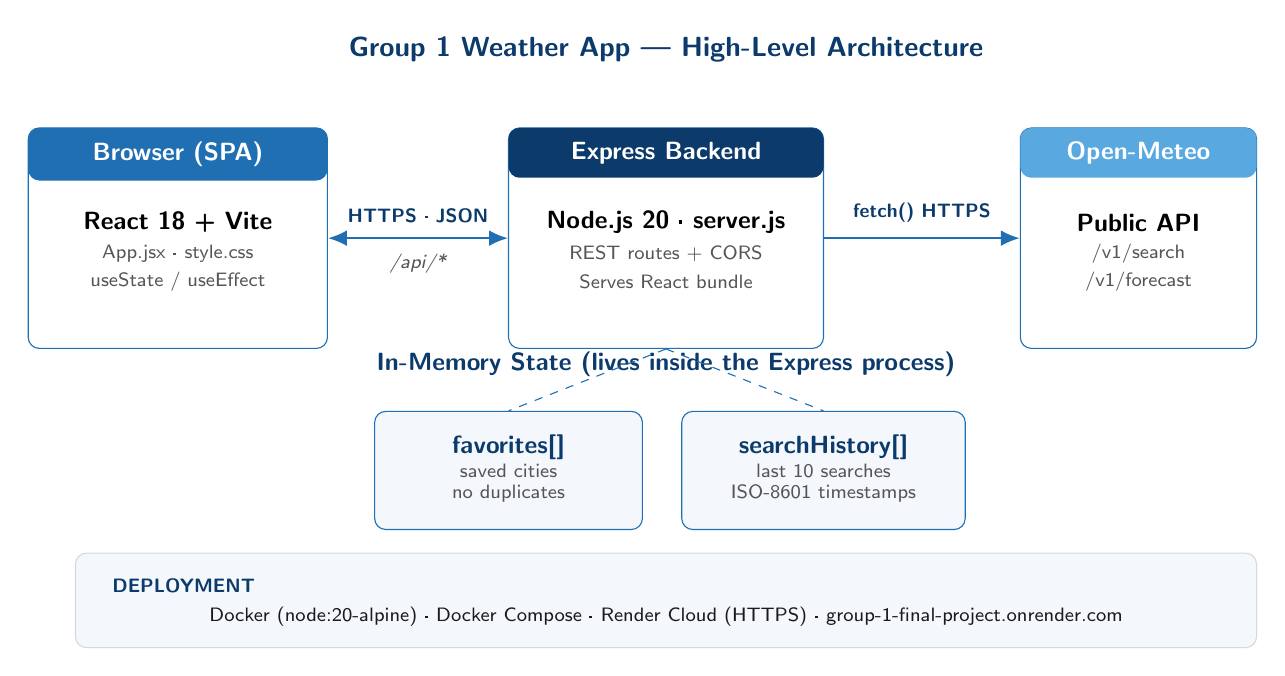
\begin{tikzpicture}[x=1cm,y=1cm]
  \node[font=\bfseries, text=brandNavy] at (0,4.4) {Group 1 Weather App --- High-Level Architecture};

  \node[box, minimum width=3.8cm, minimum height=2.8cm] (browser) at (-6.2,2) {};
  \node[boxblue, minimum width=3.8cm, anchor=north] at (browser.north) {Browser (SPA)};
  \node[font=\small] at ($(browser.center)+(0,0.2)$) {\textbf{React 18 + Vite}};
  \node[font=\scriptsize, text=brandMuted] at ($(browser.center)+(0,-0.2)$) {App.jsx \textperiodcentered{} style.css};
  \node[font=\scriptsize, text=brandMuted] at ($(browser.center)+(0,-0.55)$) {useState / useEffect};

  \node[box, minimum width=4.0cm, minimum height=2.8cm] (backend) at (0,2) {};
  \node[boxdark, minimum width=4.0cm, anchor=north] at (backend.north) {Express Backend};
  \node[font=\small] at ($(backend.center)+(0,0.2)$) {\textbf{Node.js 20 \textperiodcentered{} server.js}};
  \node[font=\scriptsize, text=brandMuted] at ($(backend.center)+(0,-0.2)$) {REST routes + CORS};
  \node[font=\scriptsize, text=brandMuted] at ($(backend.center)+(0,-0.55)$) {Serves React bundle};

  \node[box, minimum width=3.0cm, minimum height=2.8cm] (meteo) at (6.0,2) {};
  \node[boxsky, minimum width=3.0cm, anchor=north] at (meteo.north) {Open-Meteo};
  \node[font=\small] at ($(meteo.center)+(0,0.2)$) {\textbf{Public API}};
  \node[font=\scriptsize, text=brandMuted] at ($(meteo.center)+(0,-0.2)$) {/v1/search};
  \node[font=\scriptsize, text=brandMuted] at ($(meteo.center)+(0,-0.55)$) {/v1/forecast};

  \draw[bidirarrow] (browser.east) -- node[bluelabel, above=2pt]{HTTPS \textperiodcentered{} JSON} node[graylabel, below=2pt]{/api/*} (backend.west);
  \draw[flowarrow]  (backend.east) -- node[bluelabel, above=2pt]{fetch() HTTPS} (meteo.west);

  \node[font=\bfseries\small, text=brandNavy] at (0,0.4) {In-Memory State (lives inside the Express process)};

  \node[boxlight, minimum width=3.4cm, minimum height=1.5cm] (favs) at (-2.0,-0.95) {};
  \node[font=\bfseries\small, text=brandNavy] at ($(favs.center)+(0,0.3)$) {favorites[]};
  \node[font=\scriptsize, text=brandMuted] at ($(favs.center)+(0,0.0)$) {saved cities};
  \node[font=\scriptsize, text=brandMuted] at ($(favs.center)+(0,-0.3)$) {no duplicates};

  \node[boxlight, minimum width=3.6cm, minimum height=1.5cm] (hist) at (2.0,-0.95) {};
  \node[font=\bfseries\small, text=brandNavy] at ($(hist.center)+(0,0.3)$) {searchHistory[]};
  \node[font=\scriptsize, text=brandMuted] at ($(hist.center)+(0,0.0)$) {last 10 searches};
  \node[font=\scriptsize, text=brandMuted] at ($(hist.center)+(0,-0.3)$) {ISO-8601 timestamps};

  \draw[dashed, brandBlue] (backend.south) -- (favs.north);
  \draw[dashed, brandBlue] (backend.south) -- (hist.north);

  \node[draw=brandBorder, fill=brandLight, minimum width=15cm, minimum height=1.2cm,
        rounded corners=4pt] (deploy) at (0,-2.6) {};
  \node[anchor=north west, font=\bfseries\scriptsize, text=brandNavy]
        at ([xshift=10pt, yshift=-6pt]deploy.north west) {DEPLOYMENT};
  \node[font=\scriptsize, text=brandText] at ([yshift=-6pt]deploy.center)
    {Docker (node:20-alpine) \textperiodcentered{} Docker Compose \textperiodcentered{} Render Cloud (HTTPS) \textperiodcentered{} group-1-final-project.onrender.com};
\end{tikzpicture}
\caption{Runtime architecture and in-memory state of the Group 1 Weather App.}
\label{fig:arch}
\end{figure}


\subsection{Layered Architecture View}
The system can also be described as a stack of cooperating layers. Each layer depends only on the layer immediately below it, which keeps responsibilities localized and the code easy to navigate.


\begin{figure}[H]
\centering
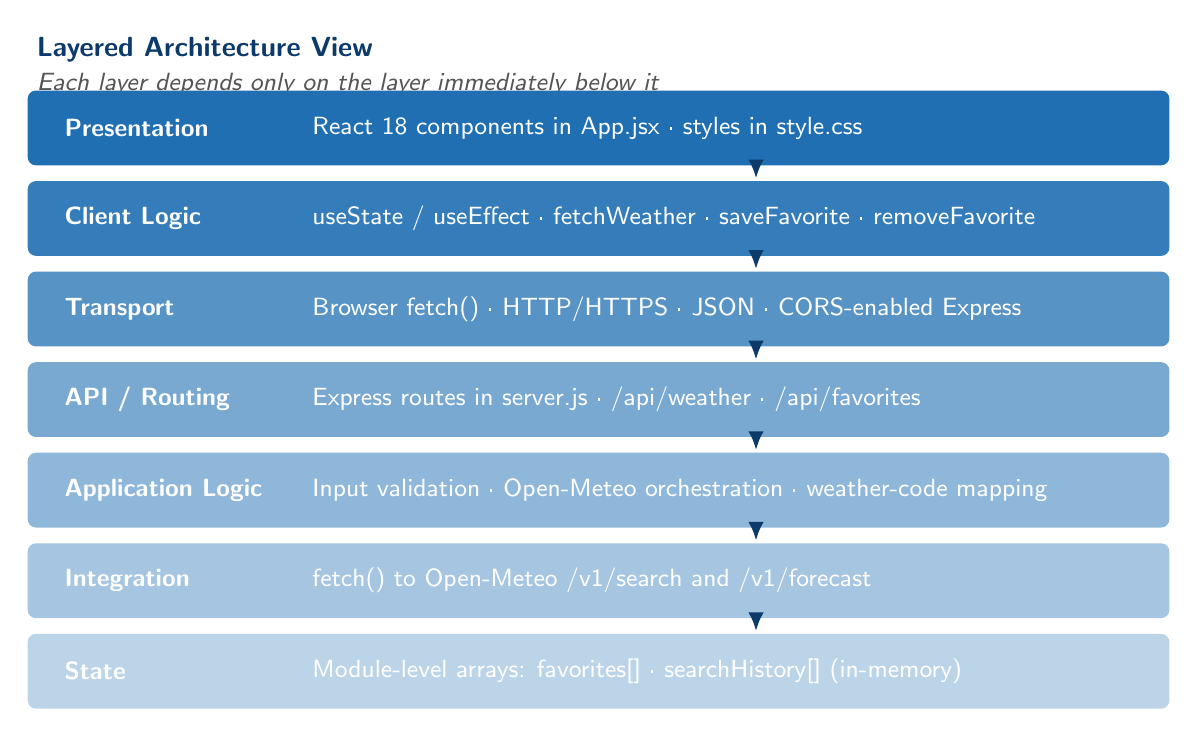
\begin{tikzpicture}
  \node[font=\bfseries, text=brandNavy, anchor=west] at (0,1.0) {Layered Architecture View};
  \node[font=\itshape\small, text=brandMuted, anchor=west] at (0,0.55) {Each layer depends only on the layer immediately below it};
  \node[rectangle, rounded corners=3pt, fill=brandBlue!100, text=white, minimum width=14.5cm, minimum height=0.95cm, anchor=west] (L0) at (0,0.00) {};
  \node[anchor=west, font=\bfseries\small, text=white] at ([xshift=10pt]L0.west) {Presentation};
  \node[anchor=west, font=\small, text=white] at ([xshift=3.5cm]L0.west) {React 18 components in App.jsx \textperiodcentered{} styles in style.css};
  \draw[->, very thick, brandNavy] ($(L0.south)+(2,0)$) -- ($(L0.south)+(2,-0.16)$);
  \node[rectangle, rounded corners=3pt, fill=brandBlue!90, text=white, minimum width=14.5cm, minimum height=0.95cm, anchor=west] (L1) at (0,-1.15) {};
  \node[anchor=west, font=\bfseries\small, text=white] at ([xshift=10pt]L1.west) {Client Logic};
  \node[anchor=west, font=\small, text=white] at ([xshift=3.5cm]L1.west) {useState / useEffect \textperiodcentered{} fetchWeather \textperiodcentered{} saveFavorite \textperiodcentered{} removeFavorite};
  \draw[->, very thick, brandNavy] ($(L1.south)+(2,0)$) -- ($(L1.south)+(2,-0.16)$);
  \node[rectangle, rounded corners=3pt, fill=brandBlue!75, text=white, minimum width=14.5cm, minimum height=0.95cm, anchor=west] (L2) at (0,-2.30) {};
  \node[anchor=west, font=\bfseries\small, text=white] at ([xshift=10pt]L2.west) {Transport};
  \node[anchor=west, font=\small, text=white] at ([xshift=3.5cm]L2.west) {Browser fetch() \textperiodcentered{} HTTP/HTTPS \textperiodcentered{} JSON \textperiodcentered{} CORS-enabled Express};
  \draw[->, very thick, brandNavy] ($(L2.south)+(2,0)$) -- ($(L2.south)+(2,-0.16)$);
  \node[rectangle, rounded corners=3pt, fill=brandBlue!60, text=white, minimum width=14.5cm, minimum height=0.95cm, anchor=west] (L3) at (0,-3.45) {};
  \node[anchor=west, font=\bfseries\small, text=white] at ([xshift=10pt]L3.west) {API / Routing};
  \node[anchor=west, font=\small, text=white] at ([xshift=3.5cm]L3.west) {Express routes in server.js \textperiodcentered{} /api/weather \textperiodcentered{} /api/favorites};
  \draw[->, very thick, brandNavy] ($(L3.south)+(2,0)$) -- ($(L3.south)+(2,-0.16)$);
  \node[rectangle, rounded corners=3pt, fill=brandBlue!50, text=white, minimum width=14.5cm, minimum height=0.95cm, anchor=west] (L4) at (0,-4.60) {};
  \node[anchor=west, font=\bfseries\small, text=white] at ([xshift=10pt]L4.west) {Application Logic};
  \node[anchor=west, font=\small, text=white] at ([xshift=3.5cm]L4.west) {Input validation \textperiodcentered{} Open-Meteo orchestration \textperiodcentered{} weather-code mapping};
  \draw[->, very thick, brandNavy] ($(L4.south)+(2,0)$) -- ($(L4.south)+(2,-0.16)$);
  \node[rectangle, rounded corners=3pt, fill=brandBlue!40, text=white, minimum width=14.5cm, minimum height=0.95cm, anchor=west] (L5) at (0,-5.75) {};
  \node[anchor=west, font=\bfseries\small, text=white] at ([xshift=10pt]L5.west) {Integration};
  \node[anchor=west, font=\small, text=white] at ([xshift=3.5cm]L5.west) {fetch() to Open-Meteo /v1/search and /v1/forecast};
  \draw[->, very thick, brandNavy] ($(L5.south)+(2,0)$) -- ($(L5.south)+(2,-0.16)$);
  \node[rectangle, rounded corners=3pt, fill=brandBlue!30, text=white, minimum width=14.5cm, minimum height=0.95cm, anchor=west] (L6) at (0,-6.90) {};
  \node[anchor=west, font=\bfseries\small, text=white] at ([xshift=10pt]L6.west) {State};
  \node[anchor=west, font=\small, text=white] at ([xshift=3.5cm]L6.west) {Module-level arrays: favorites[] \textperiodcentered{} searchHistory[] (in-memory)};
\end{tikzpicture}
\caption{Layered architecture view of the application.}
\label{fig:layers}
\end{figure}


%% ============================================================
\section{Component Design}
The implementation is naturally divided into two top-level packages, \texttt{frontend} and \texttt{backend}, each with its own \texttt{package.json}, Dockerfile, and dependency set. The subsections below describe the components contained in each package and how those components interact at runtime.

\subsection{Frontend Components}
The React frontend is a single-file SPA that exports an \texttt{App} component. Although the file is small, several logical components can be identified within it:

\begin{tabularx}{\linewidth}{| L{1.6in} | Y |}
\hline
\rowcolor{brandNavy}\thead{Component} & \thead{Responsibility} \\
\hline
Hero / Search Box  & Displays the application title and the city-search input. Bound to the \texttt{city} state variable; calls \texttt{fetchWeather()} on submit. \\ \hline
\rowcolor{brandRowAlt}Current Card       & Displays the current temperature, humidity, wind speed, and condition for the resolved city. Includes the Save Favorite button. \\ \hline
Forecast Card      & Renders a five-cell grid containing each day of the five-day forecast. \\ \hline
\rowcolor{brandRowAlt}Favorites Panel    & Lists saved cities; each entry can be selected to re-fetch its weather or removed with a trash icon. \\ \hline
History Panel      & Lists the ten most recent successful searches, each with its timestamp; entries are clickable to re-fetch. \\ \hline
\rowcolor{brandRowAlt}Error / Loading Banners & Inline UI states that appear when a request is in flight or has failed. \\ \hline
\end{tabularx}

All state is managed locally with React hooks. Six pieces of state are maintained:

\begin{tabularx}{\linewidth}{| L{1.3in} | L{1.4in} | Y |}
\hline
\rowcolor{brandNavy}\thead{State} & \thead{Type} & \thead{Purpose} \\
\hline
\texttt{city}      & string         & Current value of the search input. \\ \hline
\rowcolor{brandRowAlt}\texttt{weather}   & object \textbar{} null & Last successful weather payload returned by the backend. \\ \hline
\texttt{history}   & array          & Most recent searches, returned from \texttt{/api/history}. \\ \hline
\rowcolor{brandRowAlt}\texttt{favorites} & array          & Saved favorites, returned from \texttt{/api/favorites}. \\ \hline
\texttt{error}     & string         & Last error message to display in the error banner. \\ \hline
\rowcolor{brandRowAlt}\texttt{loading}   & boolean        & Whether an \texttt{/api/weather} request is currently in flight. \\ \hline
\end{tabularx}

\subsection{Backend Components}
The Express backend is a single \texttt{server.js} module. It can be decomposed into the following logical components:

\begin{tabularx}{\linewidth}{| L{1.6in} | Y |}
\hline
\rowcolor{brandNavy}\thead{Component} & \thead{Responsibility} \\
\hline
App Bootstrap         & Imports dependencies, computes \texttt{\_\_dirname}, attaches CORS, JSON body parsing, and morgan logging. \\ \hline
\rowcolor{brandRowAlt}Static File Server    & Serves the compiled React bundle from \texttt{../frontend/dist} for production deployments. \\ \hline
Weather Code Map      & Constant lookup table that translates the integer \texttt{weather\_code} returned by Open-Meteo to a human-readable condition string. \\ \hline
\rowcolor{brandRowAlt}In-Memory Stores      & Module-level \texttt{searchHistory} and \texttt{favorites} arrays. \\ \hline
Weather Handler       & \texttt{GET /api/weather}: validates input, geocodes, fetches forecast, transforms data, records history, returns JSON. \\ \hline
\rowcolor{brandRowAlt}History Handler       & \texttt{GET /api/history}: returns the current search-history array. \\ \hline
Favorites Handlers    & \texttt{GET}, \texttt{POST}, and \texttt{DELETE} routes for the favorites list with case-insensitive de-duplication. \\ \hline
\rowcolor{brandRowAlt}SPA Fallback          & \texttt{GET *} sends \texttt{frontend/dist/index.html} so client-side routes resolve in production. \\ \hline
Listener              & \texttt{app.listen(PORT)} where \texttt{PORT} defaults to 5000 or honors \texttt{process.env.PORT} for Render. \\ \hline
\end{tabularx}

\subsection{Component Interaction (Sequence)}
The sequence diagram below summarizes how the frontend and backend components collaborate to satisfy a typical weather search. Solid arrows indicate calls; dashed arrows indicate responses.


\begin{figure}[H]
\centering
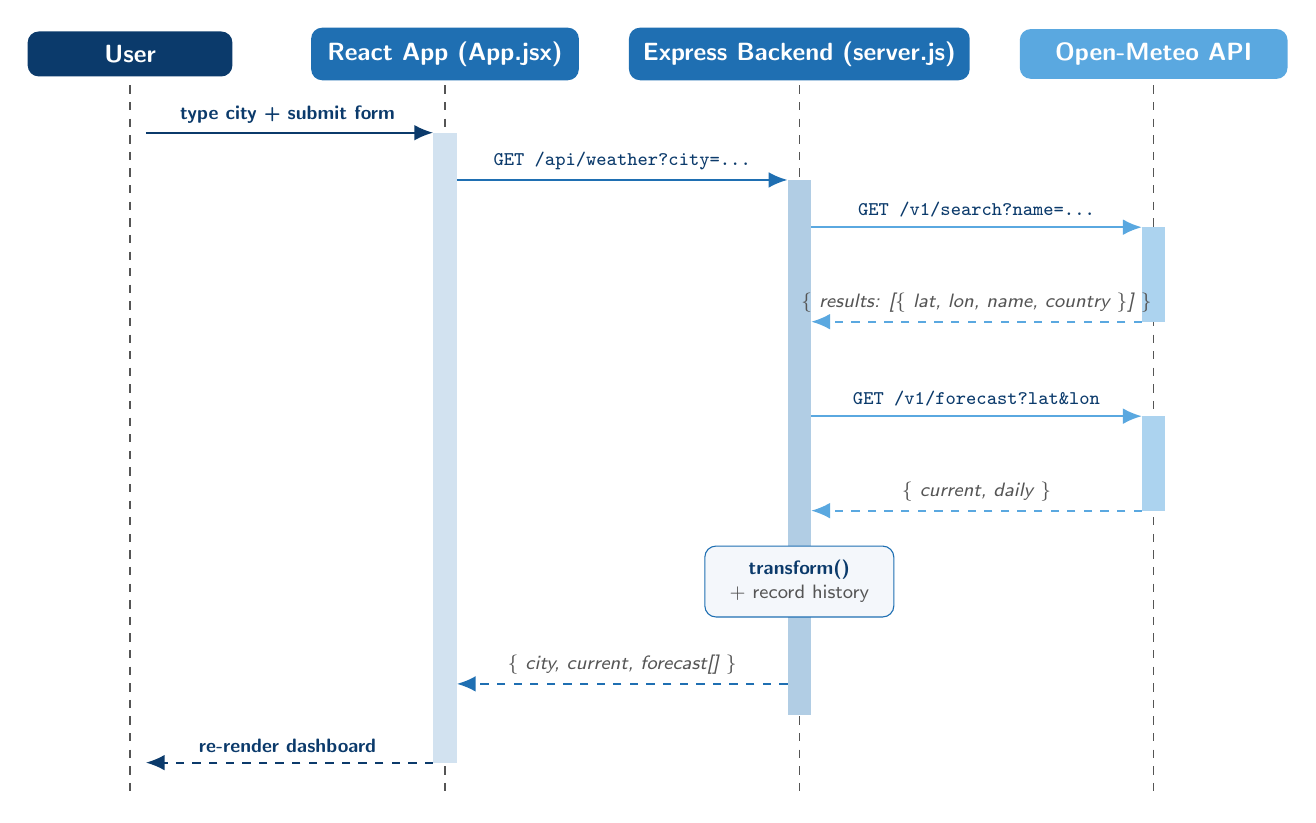
\begin{tikzpicture}[x=1cm,y=1cm]
  \node[boxdark, minimum width=2.6cm] (uH) at (0,0)    {User};
  \node[boxblue, minimum width=3.4cm] (rH) at (4,0)    {React App (App.jsx)};
  \node[boxblue, minimum width=4.0cm] (bH) at (8.5,0)  {Express Backend (server.js)};
  \node[boxsky,  minimum width=3.4cm] (mH) at (13,0)   {Open-Meteo API};

  \foreach \x in {0,4,8.5,13} {%
    \draw[dashed, brandMuted] (\x,-0.4) -- (\x,-9.4);
  }

  \fill[brandBlue!20] (3.85,-1.0) rectangle (4.15,-9.0);
  \fill[brandBlue!35] (8.35,-1.6) rectangle (8.65,-8.4);
  \fill[brandSky!50]  (12.85,-2.2) rectangle (13.15,-3.4);
  \fill[brandSky!50]  (12.85,-4.6) rectangle (13.15,-5.8);

  \draw[->, thick, brandNavy] (0.2,-1.0) -- (3.85,-1.0);
  \node[bluelabel, above] at (2.0,-1.0) {type city + submit form};

  \draw[->, thick, brandBlue] (4.15,-1.6) -- (8.35,-1.6);
  \node[font=\scriptsize\bfseries\ttfamily, text=brandNavy, above] at (6.25,-1.6) {GET /api/weather?city=...};

  \draw[->, thick, brandSky]  (8.65,-2.2) -- (12.85,-2.2);
  \node[font=\scriptsize\bfseries\ttfamily, text=brandNavy, above] at (10.75,-2.2) {GET /v1/search?name=...};

  \draw[->, thick, brandSky, dashed] (12.85,-3.4) -- (8.65,-3.4);
  \node[graylabel, above] at (10.75,-3.4) {\{ results: [\{ lat, lon, name, country \}] \}};

  \draw[->, thick, brandSky]  (8.65,-4.6) -- (12.85,-4.6);
  \node[font=\scriptsize\bfseries\ttfamily, text=brandNavy, above] at (10.75,-4.6) {GET /v1/forecast?lat\&lon};

  \draw[->, thick, brandSky, dashed] (12.85,-5.8) -- (8.65,-5.8);
  \node[graylabel, above] at (10.75,-5.8) {\{ current, daily \}};

  \node[box, minimum width=2.4cm, minimum height=0.9cm, fill=brandLight] (tx) at (8.5,-6.7) {};
  \node[font=\scriptsize\bfseries, text=brandNavy] at ($(tx.center)+(0,0.15)$) {transform()};
  \node[font=\scriptsize, text=brandMuted] at ($(tx.center)+(0,-0.15)$) {+ record history};

  \draw[->, thick, brandBlue, dashed] (8.35,-8.0) -- (4.15,-8.0);
  \node[graylabel, above] at (6.25,-8.0) {\{ city, current, forecast[] \}};

  \draw[->, thick, brandNavy, dashed] (3.85,-9.0) -- (0.2,-9.0);
  \node[bluelabel, above] at (2.0,-9.0) {re-render dashboard};
\end{tikzpicture}
\caption{Component interaction sequence for a /api/weather lookup.}
\label{fig:seq}
\end{figure}


%% ============================================================
\section{Data Design}

\subsection{Data Stores}
The Group~1 Weather App does not use a persistent database. Instead, it relies on two in-memory data structures that live for the lifetime of the backend Node.js process:
\begin{itemize}
  \item \texttt{searchHistory[]} --- an array of search records, most recent first, capped at ten entries.
  \item \texttt{favorites[]} --- an array of saved city records, used as a set keyed by city name (case-insensitive).
\end{itemize}
This decision keeps the system simple and zero-config: there is no database to provision, no migration to run, and no schema to maintain. The cost is that both arrays are reset whenever the backend restarts. This is an explicit, accepted trade-off documented in Section~\ref{sec:decisions}.

\subsection{Data Structures}

\subsubsection*{Weather Response Object}
This object is constructed on every successful \texttt{/api/weather} request and returned to the client. It is the canonical contract between backend and frontend.

\begin{tabularx}{\linewidth}{| L{1.7in} | L{1.4in} | Y |}
\hline
\rowcolor{brandNavy}\thead{Field} & \thead{Type} & \thead{Source} \\
\hline
\texttt{city}                        & string              & \texttt{geoData.results[0].name} \\ \hline
\rowcolor{brandRowAlt}\texttt{country}                     & string              & \texttt{geoData.results[0].country} \\ \hline
\texttt{current.temperature}         & number (°F)         & \texttt{weatherData.current.temperature\_2m} \\ \hline
\rowcolor{brandRowAlt}\texttt{current.humidity}            & number (\%)         & \texttt{weatherData.current.relative\_humidity\_2m} \\ \hline
\texttt{current.windSpeed}           & number (mph)        & \texttt{weatherData.current.wind\_speed\_10m} \\ \hline
\rowcolor{brandRowAlt}\texttt{current.condition}           & string              & \texttt{weatherCodeMap[weatherData.current.weather\_code]} \\ \hline
\texttt{forecast[].date}             & string (YYYY-MM-DD) & \texttt{weatherData.daily.time[i]} \\ \hline
\rowcolor{brandRowAlt}\texttt{forecast[].maxTemp}          & number (°F)         & \texttt{weatherData.daily.temperature\_2m\_max[i]} \\ \hline
\texttt{forecast[].minTemp}          & number (°F)         & \texttt{weatherData.daily.temperature\_2m\_min[i]} \\ \hline
\rowcolor{brandRowAlt}\texttt{forecast[].precipitation}    & number (\%)         & \texttt{weatherData.daily.precipitation\_probability\_max[i]} \\ \hline
\texttt{forecast[].condition}        & string              & \texttt{weatherCodeMap[weatherData.daily.weather\_code[i]]} \\ \hline
\end{tabularx}

\subsubsection*{Search History Entry}
\begin{tabularx}{\linewidth}{| L{1.7in} | L{1.4in} | Y |}
\hline
\rowcolor{brandNavy}\thead{Field} & \thead{Type} & \thead{Meaning} \\
\hline
\texttt{city}       & string              & Canonical city name returned by Open-Meteo geocoding. \\ \hline
\rowcolor{brandRowAlt}\texttt{country}    & string              & Country name returned by Open-Meteo geocoding. \\ \hline
\texttt{searchedAt} & string (ISO-8601)   & Server-side timestamp at insertion: \texttt{new Date().toISOString()}. \\ \hline
\end{tabularx}

\subsubsection*{Favorite Entry}
\begin{tabularx}{\linewidth}{| L{1.7in} | L{1.4in} | Y |}
\hline
\rowcolor{brandNavy}\thead{Field} & \thead{Type} & \thead{Meaning} \\
\hline
\texttt{city}    & string & Name of the favorited city. Used as the case-insensitive primary key. \\ \hline
\rowcolor{brandRowAlt}\texttt{country} & string & Country of the favorited city. Defaults to ``Unknown'' when omitted by the client. \\ \hline
\end{tabularx}

\subsection{Level-1 Data Flow Diagram}
The diagram below shows the level-1 data flow of the system. The user interacts with four primary processes: Search Weather, Manage Favorites, View History, and View Dashboard. Each process reads from or writes to one or both of the in-memory data stores and, for the search process, also reads from Open-Meteo.


\begin{figure}[H]
\centering
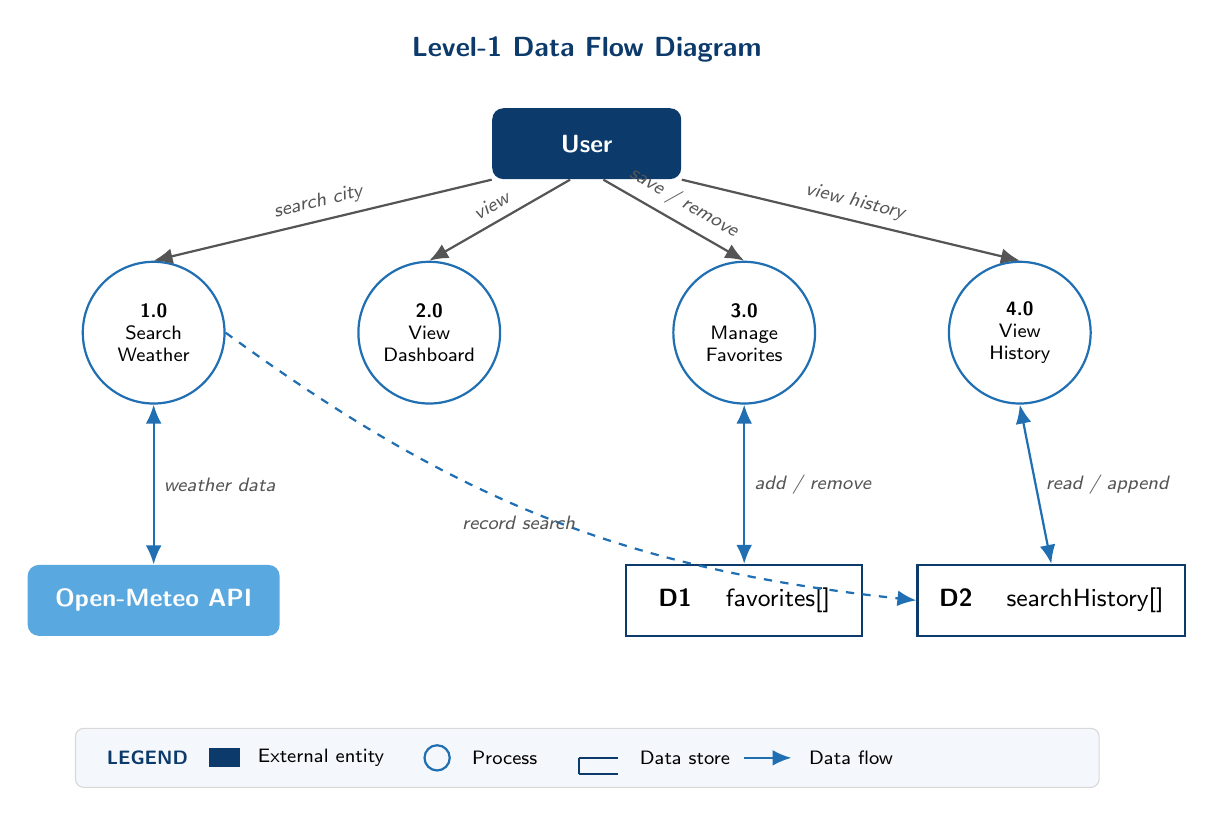
\begin{tikzpicture}[x=1cm,y=1cm]
  \node[font=\bfseries, text=brandNavy] at (7,5.6) {Level-1 Data Flow Diagram};

  \node[boxdark, minimum width=2.4cm, minimum height=0.9cm] (user) at (7,4.4) {User};

  \node[process] (p1) at (1.5,2)  {\textbf{1.0}\\Search\\Weather};
  \node[process] (p2) at (5.0,2)  {\textbf{2.0}\\View\\Dashboard};
  \node[process] (p3) at (9.0,2)  {\textbf{3.0}\\Manage\\Favorites};
  \node[process] (p4) at (12.5,2) {\textbf{4.0}\\View\\History};

  \draw[->, thick, brandMuted] (user.south west) -- node[graylabel,sloped,above]{search city}  (p1.north);
  \draw[->, thick, brandMuted] ([xshift=-6pt]user.south) -- node[graylabel,sloped,above]{view}  (p2.north);
  \draw[->, thick, brandMuted] ([xshift=6pt]user.south)  -- node[graylabel,sloped,above]{save / remove} (p3.north);
  \draw[->, thick, brandMuted] (user.south east) -- node[graylabel,sloped,above]{view history} (p4.north);

  \node[boxsky, minimum width=3.2cm, minimum height=0.9cm] (meteo) at (1.5,-1.4) {Open-Meteo API};
  \node[store, minimum width=3.0cm] (d1) at (9.0,-1.4)  {\textbf{D1} \quad favorites[]};
  \node[store, minimum width=3.4cm] (d2) at (12.9,-1.4) {\textbf{D2} \quad searchHistory[]};

  \draw[<->, thick, brandBlue] (p1.south) -- node[graylabel,right]{weather data} (meteo.north);
  \draw[<->, thick, brandBlue] (p3.south) -- node[graylabel,right]{add / remove}  (d1.north);
  \draw[<->, thick, brandBlue] (p4.south) -- node[graylabel,right]{read / append} (d2.north);
  \draw[->, thick, brandBlue, dashed] (p1.east) to[bend right=15]
        node[graylabel,below,pos=0.45]{record search} (d2.west);

  \node[draw=brandBorder, fill=brandLight, rounded corners=3pt,
        minimum width=13cm, minimum height=0.75cm, anchor=west] (leg) at (0.5,-3.4) {};
  \node[anchor=west, font=\bfseries\scriptsize, text=brandNavy] at ([xshift=8pt]leg.west) {LEGEND};
  \fill[brandNavy] ([xshift=1.7cm,yshift=-0.12cm]leg.west) rectangle ++(0.4,0.24);
  \node[anchor=west, font=\scriptsize] at ([xshift=2.2cm]leg.west) {External entity};
  \draw[brandBlue, thick] ([xshift=4.6cm]leg.west) circle (0.16);
  \node[anchor=west, font=\scriptsize] at ([xshift=4.92cm]leg.west) {Process};
  \draw[brandNavy, thick] ([xshift=6.4cm]leg.west) -- ++(0.5,0);
  \draw[brandNavy, thick] ([xshift=6.4cm,yshift=-0.2cm]leg.west) -- ++(0.5,0);
  \draw[brandNavy, thick] ([xshift=6.4cm]leg.west) -- ++(0,-0.2);
  \node[anchor=west, font=\scriptsize] at ([xshift=7.05cm]leg.west) {Data store};
  \draw[->, thick, brandBlue] ([xshift=8.5cm]leg.west) -- ++(0.6,0);
  \node[anchor=west, font=\scriptsize] at ([xshift=9.2cm]leg.west) {Data flow};
\end{tikzpicture}
\caption{Level-1 data flow diagram showing processes, data stores, and the external entity.}
\label{fig:dfd}
\end{figure}


%% ============================================================
\section{Interface Design}

\subsection{Backend REST API}
The backend exposes the following REST endpoints. All endpoints accept and return \texttt{application/json} and are mounted under the \texttt{/api} prefix.

\renewcommand{\arraystretch}{1.25}
\begin{longtable}{| C{0.55in} | L{1.5in} | L{1.3in} | L{1.6in} | L{0.95in} |}
\hline
\rowcolor{brandNavy}\thead{Method} & \thead{Path} & \thead{Request} & \thead{Response (success)} & \thead{Errors} \\
\hline
\endfirsthead
\hline
\rowcolor{brandNavy}\thead{Method} & \thead{Path} & \thead{Request} & \thead{Response (success)} & \thead{Errors} \\
\hline
\endhead
\texttt{GET}    & \texttt{/api/weather}        & Query: \texttt{?city=\textlangle name\textrangle} & 200 --- weather response object (see \S4.2). & 400 if city missing; 404 if not found; 500 on upstream failure. \\ \hline
\rowcolor{brandRowAlt}\texttt{GET}    & \texttt{/api/history}        & ---                                                & 200 --- array of search-history entries (most recent first, $\leq$10). & --- \\ \hline
\texttt{GET}    & \texttt{/api/favorites}      & ---                                                & 200 --- array of favorite entries.                  & --- \\ \hline
\rowcolor{brandRowAlt}\texttt{POST}   & \texttt{/api/favorites}      & Body: \texttt{\{ city, country? \}}                & 200 --- updated favorites array.                    & 400 if city missing. \\ \hline
\texttt{DELETE} & \texttt{/api/favorites/:city}& Path param: city name                              & 200 --- updated favorites array.                    & --- \\ \hline
\rowcolor{brandRowAlt}\texttt{GET}    & \texttt{*}                   & Any non-API path                                   & 200 --- \texttt{frontend/dist/index.html} (SPA fallback). & --- \\ \hline
\end{longtable}

\subsection{External API Integration}
The backend integrates with two Open-Meteo endpoints. Geocoding is called first to resolve the user-supplied city name to coordinates. The forecast endpoint is then called with those coordinates plus a curated list of variables and unit overrides.

\begin{codeblock}
// Geocoding
GET https://geocoding-api.open-meteo.com/v1/search
    ?name={city}&count=1&language=en&format=json

// Forecast
GET https://api.open-meteo.com/v1/forecast
    ?latitude={lat}
    &longitude={lon}
    &current=temperature_2m,relative_humidity_2m,weather_code,wind_speed_10m
    &daily=weather_code,temperature_2m_max,temperature_2m_min,
           precipitation_probability_max
    &temperature_unit=fahrenheit
    &wind_speed_unit=mph
    &timezone=auto
\end{codeblock}

\subsection{User Interface Design}
The UI is intentionally focused: one search box, two informational cards (current and forecast), and two side panels (favorites and history). The page uses a soft gradient background, rounded card corners, and a single accent color (\texttt{\#2563eb}) for the primary action and key highlights. The layout uses CSS Grid for the main dashboard and the forecast row; below 850 pixels of viewport width, all multi-column areas collapse to a single column for mobile readability.

The visual hierarchy from top to bottom is:
\begin{itemize}
  \item Hero header --- title + tagline on the left, search box on the right.
  \item Error banner and loading banner --- appear when applicable, beneath the hero.
  \item Dashboard --- current-weather card (left) and forecast card (right).
  \item Side sections --- favorites panel (left) and search history panel (right).
\end{itemize}

%% ============================================================
\section{Detailed Module Design}

\subsection{Backend: server.js}
\texttt{server.js} is the single backend module. Its responsibilities, in order of declaration, are:
\begin{itemize}
  \item Import \texttt{express}, \texttt{cors}, \texttt{morgan}, \texttt{path}, and \texttt{fileURLToPath} from Node's URL module.
  \item Create the Express app, attach CORS, JSON body parsing, and morgan request logging.
  \item Serve compiled frontend assets through \texttt{express.static("../frontend/dist")}.
  \item Declare the \texttt{weatherCodeMap} lookup table that maps Open-Meteo integer codes to human strings.
  \item Declare module-level \texttt{searchHistory[]} and \texttt{favorites[]} arrays.
  \item Register the five \texttt{/api} routes.
  \item Register the SPA fallback route (\texttt{app.get("*")}).
  \item Start listening on \texttt{process.env.PORT} or 5000.
\end{itemize}

\subsubsection*{Pseudocode --- GET /api/weather}
\begin{codeblock}
function handleWeather(req, res):
    city = req.query.city
    if city is empty:
        return 400 { error: "City is required" }

    geo = await fetch(open-meteo geocoding for city)
    if geo.results is empty:
        return 404 { error: "City not found" }

    location = geo.results[0]
    weather  = await fetch(open-meteo forecast for location.lat, location.lon)

    result = transform(location, weather)         // see  4.2

    searchHistory.unshift({
        city: result.city, country: result.country,
        searchedAt: now().toISOString()
    })
    searchHistory = searchHistory.slice(0, 10)

    return 200 result

    on any thrown error:
        return 500 { error: "Failed to fetch weather data" }
\end{codeblock}

\subsubsection*{Pseudocode --- POST /api/favorites}
\begin{codeblock}
function addFavorite(req, res):
    { city, country } = req.body
    if city is empty:
        return 400 { error: "City is required" }

    exists = favorites.some(f => f.city.toLowerCase() === city.toLowerCase())
    if not exists:
        favorites.push({ city, country: country or "Unknown" })

    return 200 favorites
\end{codeblock}

\subsection{Frontend: App.jsx}
\texttt{App.jsx} is the single frontend module. It defines a functional component, \texttt{App}, and mounts it into the \texttt{\#root} element. Its structure is:
\begin{itemize}
  \item Import React hooks, lucide-react icons, \texttt{createRoot}, and the local style sheet.
  \item Define the \texttt{App} component with six pieces of state (city, weather, history, favorites, error, loading).
  \item Define async data functions: \texttt{fetchWeather}, \texttt{fetchHistory}, \texttt{fetchFavorites}, \texttt{saveFavorite}, \texttt{removeFavorite}.
  \item Run \texttt{useEffect} on mount to pre-load weather for Los Angeles plus the current favorites and history.
  \item Return JSX for the hero, dashboard, and side sections, with conditional banners for loading and errors.
  \item Bootstrap the app at the bottom of the file: \texttt{createRoot(document.getElementById("root")).render(<App />)}.
\end{itemize}

\subsubsection*{Pseudocode --- fetchWeather()}
\begin{codeblock}
async function fetchWeather(searchCity = city):
    setLoading(true)
    setError("")
    try:
        response = await fetch("/api/weather?city=" + encode(searchCity))
        data     = await response.json()
        if !response.ok:
            throw new Error(data.error or "Weather request failed")
        setWeather(data)
        setCity(data.city)
        fetchHistory()
    catch err:
        setError(err.message)
        setWeather(null)
    finally:
        setLoading(false)
\end{codeblock}

%% ============================================================
\section{Deployment Design}
Both the frontend and the backend are packaged as Docker images and orchestrated locally with Docker Compose. Each service has its own Dockerfile built on top of the official \texttt{node:20-alpine} image, and the \texttt{docker-compose.yml} file exposes the appropriate ports and declares that the frontend depends on the backend. The deployed instance is hosted on Render at \texttt{https://group-1-final-project.onrender.com}. The diagram below shows the deployment topology in both local and production modes.


\begin{figure}[H]
\centering
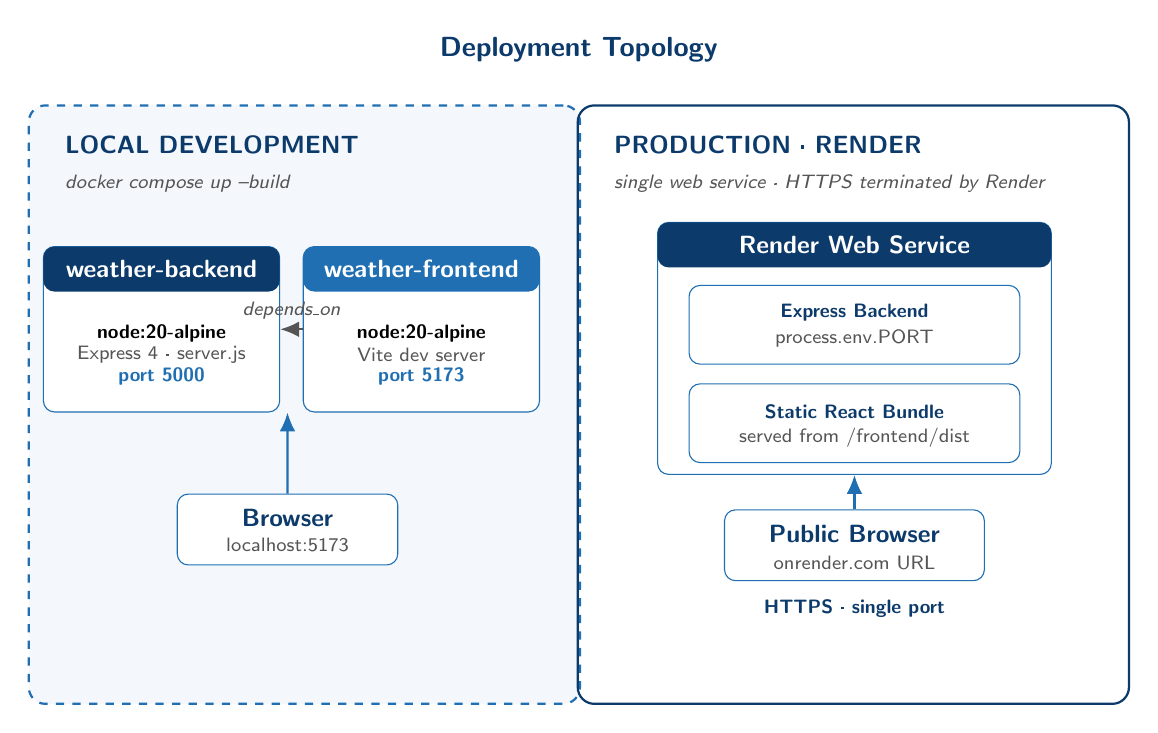
\begin{tikzpicture}[x=1cm,y=1cm]
  \node[font=\bfseries, text=brandNavy] at (7,5.5) {Deployment Topology};

  \node[draw=brandBlue, dashed, thick, rounded corners=6pt, fill=brandLight,
        minimum width=7cm, minimum height=7.6cm, anchor=north west] (local) at (0,4.8) {};
  \node[anchor=north west, font=\bfseries\small, text=brandNavy]
        at ([xshift=10pt, yshift=-8pt]local.north west) {LOCAL DEVELOPMENT};
  \node[anchor=north west, font=\itshape\scriptsize, text=brandMuted]
        at ([xshift=10pt, yshift=-22pt]local.north west) {docker compose up --build};

  \node[box, minimum width=3cm, minimum height=2.1cm, anchor=north] (be) at (1.7,3.0) {};
  \node[boxdark, anchor=north, minimum width=3cm] at (be.north) {weather-backend};
  \node[font=\scriptsize] at ($(be.center)+(0,-0.05)$) {\textbf{node:20-alpine}};
  \node[font=\scriptsize, text=brandMuted] at ($(be.center)+(0,-0.32)$) {Express 4 \textperiodcentered{} server.js};
  \node[font=\scriptsize\bfseries, text=brandBlue] at ($(be.center)+(0,-0.6)$) {port 5000};

  \node[box, minimum width=3cm, minimum height=2.1cm, anchor=north] (fe) at (5.0,3.0) {};
  \node[boxblue, anchor=north, minimum width=3cm] at (fe.north) {weather-frontend};
  \node[font=\scriptsize] at ($(fe.center)+(0,-0.05)$) {\textbf{node:20-alpine}};
  \node[font=\scriptsize, text=brandMuted] at ($(fe.center)+(0,-0.32)$) {Vite dev server};
  \node[font=\scriptsize\bfseries, text=brandBlue] at ($(fe.center)+(0,-0.6)$) {port 5173};

  \draw[->, thick, brandMuted] (fe.west) -- node[graylabel,above]{depends\_on} (be.east);

  \node[box, minimum width=2.8cm, minimum height=0.9cm] (lbrow) at (3.3,-0.6) {};
  \node[font=\small\bfseries, text=brandNavy] at ($(lbrow.center)+(0,0.15)$) {Browser};
  \node[font=\scriptsize, text=brandMuted] at ($(lbrow.center)+(0,-0.2)$) {localhost:5173};
  \draw[->, thick, brandBlue] (lbrow.north) -- ($(fe.south)+(-1.7,0)$);

  \node[draw=brandNavy, thick, rounded corners=6pt,
        minimum width=7cm, minimum height=7.6cm, anchor=north east] (prod) at (14,4.8) {};
  \node[anchor=north west, font=\bfseries\small, text=brandNavy]
        at ([xshift=10pt, yshift=-8pt]prod.north west) {PRODUCTION \textperiodcentered{} RENDER};
  \node[anchor=north west, font=\itshape\scriptsize, text=brandMuted]
        at ([xshift=10pt, yshift=-22pt]prod.north west) {single web service \textperiodcentered{} HTTPS terminated by Render};

  \node[box, minimum width=5cm, minimum height=3.2cm, anchor=center] (svc) at (10.5,1.7) {};
  \node[boxdark, anchor=north, minimum width=5cm] at (svc.north) {Render Web Service};

  \node[box, minimum width=4.2cm, minimum height=1.0cm, anchor=center] (be2) at (10.5,2.0) {};
  \node[font=\scriptsize\bfseries, text=brandNavy] at ($(be2.center)+(0,0.15)$) {Express Backend};
  \node[font=\scriptsize, text=brandMuted] at ($(be2.center)+(0,-0.18)$) {process.env.PORT};

  \node[box, minimum width=4.2cm, minimum height=1.0cm, anchor=center] (st) at (10.5,0.75) {};
  \node[font=\scriptsize\bfseries, text=brandNavy] at ($(st.center)+(0,0.15)$) {Static React Bundle};
  \node[font=\scriptsize, text=brandMuted] at ($(st.center)+(0,-0.18)$) {served from /frontend/dist};

  \node[box, minimum width=3.3cm, minimum height=0.9cm] (pbrow) at (10.5,-0.8) {};
  \node[font=\small\bfseries, text=brandNavy] at ($(pbrow.center)+(0,0.15)$) {Public Browser};
  \node[font=\scriptsize, text=brandMuted] at ($(pbrow.center)+(0,-0.22)$) {onrender.com URL};
  \draw[->, thick, brandBlue] (pbrow.north) -- (svc.south);
  \node[font=\scriptsize\bfseries, text=brandNavy] at (10.5,-1.6) {HTTPS \textperiodcentered{} single port};
\end{tikzpicture}
\caption{Deployment topology: local Docker Compose vs.\ production Render service.}
\label{fig:deploy}
\end{figure}


\subsubsection*{docker-compose.yml}
\begin{codeblock}
services:
  backend:
    build: ./backend
    container_name: weather-backend
    ports: ["5000:5000"]

  frontend:
    build: ./frontend
    container_name: weather-frontend
    ports: ["5173:5173"]
    depends_on:
      - backend
\end{codeblock}

During development the two services run as separate containers and the frontend's Vite dev server proxies API calls to the backend container. In production, the backend additionally serves the compiled frontend bundle as static assets so that the entire application can be exposed behind a single port.

%% ============================================================
\section{Testing Strategy}
Testing for the Group~1 Weather App was driven through TestRail across four snapshot cycles. Each snapshot focused on a distinct slice of the system, and the final test run validated the full integrated product.

\begin{tabularx}{\linewidth}{| L{1in} | L{1.7in} | Y |}
\hline
\rowcolor{brandNavy}\thead{Snapshot} & \thead{Focus} & \thead{Representative Test Coverage} \\
\hline
Snapshot~1 & Project setup                  & Repository structure, dependency installation, baseline frontend and backend skeletons. \\ \hline
\rowcolor{brandRowAlt}Snapshot~2 & Core search functionality       & Open-Meteo integration, valid and invalid city searches, current weather, and five-day forecast rendering. \\ \hline
Snapshot~3 & Favorites and history          & Adding favorites, preventing duplicates, removing favorites, populating and capping the search history. \\ \hline
\rowcolor{brandRowAlt}Snapshot~4 & Containerization and deployment & Docker build and run for both services, docker-compose startup, and live deployment validation on Render. \\ \hline
\end{tabularx}

In addition to scripted TestRail cases, the following error scenarios were exercised manually during development: empty city input, non-existent city names, dropped network connectivity, and forced backend restarts. The backend's error responses (400, 404, 500) are surfaced to the user through the frontend's red error banner.

%% ============================================================
\section{Design Decisions and Rationale}\label{sec:decisions}
Several design decisions deserve explicit discussion because they shape the simplicity and limitations of the system.

\subsubsection*{Single-page application instead of multi-page routing}
All UI is rendered from a single React \texttt{App} component. The application has only one screen, so introducing a router would have added complexity with no user-facing benefit. The single component also keeps state co-located and easy to follow.

\subsubsection*{In-memory state instead of a database}
Favorites and history live in module-level arrays inside the Express process. This eliminates the need to provision and migrate a database, which would have been disproportionate to a class project at this scale. The trade-off is that both lists reset on every backend restart, which is acceptable because no entry contains personally identifiable information and the data is easily reproduced by the user.

\subsubsection*{Backend proxy instead of direct calls from the browser}
The browser never calls Open-Meteo directly. Instead, the React frontend always calls the backend, which in turn calls Open-Meteo. This keeps the response shape consistent and frontend-friendly, allows the system to add server-side concerns (logging, history recording, weather-code translation) in one place, and shields the client from changes in the upstream API.

\subsubsection*{Open-Meteo as the weather provider}
Open-Meteo was selected because it is free, requires no API key, and exposes both geocoding and forecast endpoints with the granularity needed for this project (current values plus daily aggregates including precipitation probability). Other providers were considered but rejected because they required paid plans or rate-limited free tiers.

\subsubsection*{Docker + Render for deployment}
Containerization with Docker ensures that ``works on my machine'' is the same as ``works in production''. Render was chosen as the deployment target because its free tier accepts Node.js services with public HTTPS termination and because \texttt{process.env.PORT} is honored automatically, which matches the existing \texttt{server.js} bootstrap.

\end{document}
